\documentclass[12pt,a4paper,oneside]{book}
\usepackage[utf8]{inputenc}
\usepackage[spanish,es-tabla]{babel}
\usepackage{graphicx}
\usepackage{parskip}
\usepackage[acronym,nonumberlist,toc]{glossaries}
\usepackage[colorlinks=true,urlcolor=blue,citecolor=blue]{hyperref}
\usepackage{float}
\usepackage{makecell}
\usepackage{geometry}
\geometry{
  a4paper,
  left=2.5cm,top=1cm,right=2.5cm,bottom=2cm,
  headheight=2.5cm,headsep=1cm,foot=1cm,footskip=1cm,
  includeheadfoot
}
\usepackage{pdfpages}
\usepackage{fancyhdr} %Encabezado y pie de página
\usepackage{lastpage} 
\usepackage[acronym,nonumberlist,toc]{glossaries}
\usepackage[
backend=biber,
style=numeric,
sorting=nyt
]{biblatex}
\usepackage{csquotes}                   %Para que no salte el warning, biblatex + babel
\usepackage{bold-extra}                 %Para que no salte warning de fuentes

\addbibresource{bibliografia.bib}

\makeglossaries
\newacronym{afua}{AFUA}{Advanced Flexible Use of Airspace}
\newacronym{cdm}{CDM}{Colaborative Decisión Making}
\newacronym{swim}{SWIM}{System Wide Information Management}
\newacronym{ocd}{OCD}{Operational Concept Document}
\newacronym{atm}{ATM}{Air Traffic Management}
\newacronym{asm}{ASM}{Air Space Management}
\newacronym{atfcm}{ATFCM}{Air  Traffic  Flow  and  Capacity  Management}
\newacronym{ats}{ATS}{Air Traffic Services}
\newacronym{dac}{DAC}{Dynamic Airspace Configuration}
\newacronym{dcb}{DCB}{Demand Capacity Balancing}
\newacronym{sesar}{SESAR}{Single European Sky ATM Research}
\newacronym{ceac}{CEAC}{ Conferencia Europea de Aviación Civil}
\newacronym{fua}{FUA}{Flexible Use of Airspace}
\newacronym{oat}{Operational Air Traffic}{OAT}
\newacronym{gat}{General Air Traffic}{GAT}
\newacronym{fir}{FIR}{Flight Information Region, Región de Información de Vuelo}
\newacronym{vpa}{VPA}{Variable Profile Area}
\newacronym{dma}{DMA}{Dynamic Mobile Area}
\newacronym{fra}{FRA}{Free Route Airspace}
\newacronym{fab}{FAB}{Functional Airspace Block}
\newacronym{oaci}{OACI}{Organización de la Aviación Civil Internacional}
\newacronym{eurocontrol}{Eurocontrol}{Organización Europea para la Seguridad de la Navegación Aérea}
\newacronym{aiaa}{AIAA}{American Institute of Aeronautics and Astronautics}
\newacronym{ernip}{ERNIP}{European  Route  Network  Improvement  Plan}
\newacronym{ce}{CE}{Comisión Europea}
\newacronym{pbn}{PBN}{Perfomance Based Navigation}
\newacronym{gnss}{GNSS}{Global Navigation Satellite System}
\newacronym{ils}{ILS}{Instrumental Landing System, Sistema de Aterrizaje Instrumental}
\newacronym{mls}{MLS}{Microwave Landing System}
\glsaddall

\setlength{\parskip}{\baselineskip}		
\renewcommand\theadfont{\bfseries}
\emergencystretch=1em                   %Quita los warning hbox

\setcounter{secnumdepth}{3}				%Se numera hasta las subsecciones
\setcounter{tocdepth}{3}       			%Índice tiene en cuenta hasta las subsubsecciones
\newcommand{\sectionbreak}{\clearpage}	%Section en página nueva

%Bloque de fancy para frontmatter distinto al mainmatter
\pagestyle{fancy}						%Defino mi estilo con el paquete fancy
\fancyhf{}								%Borro todo lo que viene por defecto, lo dejo limpio
%Encabezado con los logos
\fancyhead[R]{
\includegraphics[height=2cm]{logos/Logo_SATAA.png}}
\fancyhead[L]{
\includegraphics[height=2cm]{logos/Logo_UPM.png}}
%Pie de página
\fancyfoot[L]{Advanced Flexible Use of Airspace}
\fancyfoot[R]{\thepage}
\renewcommand{\headrulewidth}{1pt}      % Grosor linea encabezado
\renewcommand{\footrulewidth}{1pt}      % Grosor linea pie

\fancypagestyle{plain}{					%Para cambiar las páginas de capítulo
	\fancyhf{}							%limpio
	\fancyfoot[L]{Advanced Flexible Use of Airspace}
    \fancyfoot[R]{\thepage}
	\renewcommand{\headrulewidth}{0pt}	%Quito la linea de arriba en los capitulos	
}

\begin{document}
\begin{titlepage}
\centering
{
\includegraphics[width=0.5\textwidth]{logos/UPM}\par}
\vspace{0.1cm}
{\bfseries\LARGE Universidad Politécnica de Madrid \par}
\vspace{0.5cm}
{\scshape\large ESCUELA TÉCNICA SUPERIOR DE INGENIERÍA AERONÁUTICA Y DEL ESPACIO \par}
\vspace{0.25cm}
{
\includegraphics[width=0.38\textwidth]{logos/ETSIAE} \par}
\vspace{1cm}
{\scshape\Large  Gestión de áreas de otros usos. Advanced FUA Mínima automatización \par}
\vspace{0.7cm}
{\itshape\large Evolución de los conceptos ATM \par}
\vfill
{\Large Autores: \par}
{\large Cristea, Ciprian \\ Gutiérrez Teuler, Guillermo \\ Martínez Fernández, Íñigo \\ Maxence, Gallian \par}
\vfill
{\Large 20 de Octubre de 2021 \par}
\end{titlepage}

\frontmatter

%Índice para que salga el resto de índices
{\hypersetup{linkcolor=black}		%Cambio el color de los link a negro para que no me salga todo en rojo
	\tableofcontents
	\cleardoublepage
	\addcontentsline{toc}{chapter}{\listfigurename}\listoffigures
	\cleardoublepage
	\addcontentsline{toc}{chapter}{\listtablename}\listoftables
}

\printglossary[type=\acronymtype,title=Acrónimos,toctitle=Acrónimos]

\pagestyle{fancy}						%Defino mi estilo con el paquete fancy
\fancyhf{}								%Borro todo lo que viene por defecto, lo dejo limpio
%Encabezado con los logos
\fancyhead[R]{
\includegraphics[height=2cm]{logos/Logo_SATAA.png}}
\fancyhead[L]{
\includegraphics[height=2cm]{logos/Logo_UPM.png}}
%Pie de página
\fancyfoot[L]{Advanced Flexible Use of Airspace}
\fancyfoot[R]{\thepage/{\hypersetup{linkcolor=black}\pageref{LastPage}}}
\renewcommand{\headrulewidth}{1pt}      % Grosor linea encabezado
\renewcommand{\footrulewidth}{1pt}      % Grosor linea pie

\mainmatter

\chapter{Introducción}

\section{Identificación}

\textbf{Identificación:} Por asignar

\textbf{Título:} Advanced Flexible Use of Airspace 

\section{Propósito del sistema}

El motivo fundamental para plantear la implementación del \acrfull{afua} es conseguir un aumento de la capacidad en el sistema de gestión del tránsito aéreo. 

En los años previos al estallido de la pandemia, se ha comprobado que el sistema actual no va a ser capaz de absorber al aumento de la demanda, lo que provoca elevados valores de demora. Especialmente preocupante es el caso de los países europeos, donde debido a la gran cantidad de delegaciones existentes, el modelo actual está lejos de una organización óptima. 

Teniendo en cuenta que el volumen de tráfico volverá a sus valores de crecimiento anteriores una vez superados los efectos de la crisis sanitaria, se deben orientar las propuestas hacia una mejor utilización de todos los elementos implicados en las operaciones de tránsito aéreo. 

El concepto de \acrlong{afua}, permitirá mitigar los problemas derivados del uso compartido del espacio aéreo civil-militar. Esto permitirá dotar a las aeronaves de una mayor flexibilidad a la hora de maniobrar en un espacio aéreo tan congestionado como el europeo. 

En el espacio aéreo europeo se pueden encontrar diferentes tipos de usuarios, cada uno de ellos con unas necesidades de operación distintas. AFUA tratará de organizar el espacio aéreo de manera flexible para conseguir una mejor coordinación de las operaciones.

Los distintos usuarios que harán uso del espacio aéreo son:

\begin{itemize}
    \item Operaciones militares.
    \item Aviación comercial.
    \item Aviación general.
    \item Escuelas de vuelo.
    \item RPAS.
\end{itemize}

A lo largo del documento se hará referencia en múltiples ocasiones a la coordinación civil–militar. Dentro de las operaciones denominadas como civiles, encontraremos aquellas cuyo propósito no esté directamente relacionado con el entorno militar, por tanto, estarán englobadas dentro de esta categoría tanto la aviación comercial, como la aviación general y las escuelas de vuelo. Las operaciones con RPAS, se englobarán dentro del ámbito civil o del militar en función de la misión que lleven asociada.

Se debe tener en cuenta que nos encontramos dentro de un entorno muy dinámico, y que pueden surgir nuevos usuarios que necesiten hacer uso del espacio aéreo. Recientemente ha sucedido con los RPAS, que durante los últimos años han empezado a obtener una mayor relevancia, y que en el futuro serán un actor clave a la hora de organizar el espacio aéreo, puesto que ofrecen una gran versatilidad a la hora de plantear operaciones.

En el AFUA al haber nuevos usuarios en el sistema y diseñarlo de tal forma que en el futuro se puedan añadir más surge el problema de los conflictos entre usuarios. Puede ocurrir que haya conflictos entre operaciones o misiones de dos usuarios distintos de la red. Esto lleva al problema de la prioridad, hay que decidir quién la tiene y sobre quién. En este trabajo no se va a entrar en detalle ya que habría que analizar toda la casuística lo cual se escapa del alcance del actual informe. 

Se establece que todos los conflictos de prioridad entre usuarios van a ser resueltos por la organización del AFUA, ya sea a nivel regional o al más alto nivel, especialmente necesario cuando los conflictos involucran a varios países. Para establecer quién tiene prioridad el personal de la red que analiza las peticiones de los usuarios establecerá la criticidad de las operaciones que lo requieran. Por defecto las operaciones que no sean críticas serán las que tengan que adaptarse a las que se califiquen como criticas. Para facilitar ya agilizar el trabajo también se podrá llegar a acuerdos con organizaciones de usuarios. Por ejemplo, se puede llegar a un trato con el ejército nacional que en el caso que tengan que realizar una salida de urgencia ellos lo puedan declarar en el sistema y automáticamente se les asigne la máxima prioridad.

Es evidente que la implementación de este sistema debe ir asociada a grandes mejoras en otras partes del sistema. La relación del AFUA con elementos como el sistema de \acrfull{cdm}, la implementación de un sistema Free Route y el \acrfull{swim} será fundamental a la hora de plantear su desarrollo. 

\section{Alcance del OCD}

Para lograr una aplicación impecable del concepto AFUA desde la planificación estratégica hasta la resolución táctica se necesita:

\begin{itemize}
    \item Reforzar el proceso de coordinación entre todos los socios del ATM.
    \item Mejorar el mecanismo de planificación y gestión de las rutas, la sectorización asociada y las reservas de espacio aéreo (ARES).
    \item Acercamiento de los horizontes temporales del nivel 2 de ASM (Pre-táctico) y del ATFCM-DCB (ATFCM (Air Traffic Flow and Capacity Management) que evoluciona hacia el Demand Capacity Balancing.
    \item Extender el proceso de colaboración en tiempo real desde la solicitud de espacio aéreo hasta la fase táctica (nivel 3).
    \item Mejorar el intercambio de información y la notificación de todos los datos relacionados con AFUA.
    \item Consistencia en el procesamiento y la distribución de los planes de vuelo, tanto para las operaciones civiles como para las militares.
    \item Evaluación de la mejora del desempeño asociado a AFUA a través de un enfoque proactivo.
    \item Interoperabilidad de los sistemas gracias a estándares comunes y procesos de gestión del cambio adecuados.
    \item Arquitectura del sistema comúnmente acordada.
\end{itemize}

\section{Visión general}

El concepto de \acrfull{afua} nos introduce a las denominadas como operaciones llevadas a cabo en función del rendimiento y está basado en la gestión de las distintas configuraciones del espacio aéreo. 

Gracias a este concepto se aportarán nuevas posibilidades que permitirán un uso más flexible y dinámico de los distintos elementos del sistema. 

En resumen, se creará un proceso sin fisuras, que esté basado en el \acrfull{cdm}, con una avanzada herramienta de gestión en tiempo real de las configuraciones del espacio aéreo. Además, permitirá el flujo continuo de información entre el conjunto de actores implicados en el sistema ATM, a través de una tecnología de primer nivel desarrollada dentro de los proyectos de \acrfull{sesar}.

\section{Documentos de referencia}

\begin{itemize}
    \item \textbf{\citetitle{Eurocontrol2015AdvancedConcept}} de \citeauthor{Eurocontrol2015AdvancedConcept}  \cite{Eurocontrol2015AdvancedConcept}.
    \item \textbf{\citetitle{Eurocontrol2021EuropeanManagement}} de \citeauthor{Eurocontrol2021EuropeanManagement}  \cite{Eurocontrol2021EuropeanManagement}.
    \item \textbf{\citetitle{Eurocontrol2021FUA15.0}} de \citeauthor{Eurocontrol2021FUA15.0}  \cite{Eurocontrol2021FUA15.0}.
    \item \textbf{\citetitle{Eurocontrol2009SpecificationFUA}} de \citeauthor{Eurocontrol2009SpecificationFUA}  \cite{Eurocontrol2009SpecificationFUA}.
    \item \textbf{\citetitle{OACI2018Manual9971}} de \citeauthor{OACI2018Manual9971}  \cite{OACI2018Manual9971}.
    \item \textbf{\citetitle{OACI2021Manual10088}} de \citeauthor{OACI2021Manual10088}  \cite{OACI2021Manual10088}.
\end{itemize}

\section{Antecedentes}

Desde los años 90 la \acrfull{ceac} definió la nueva estrategia En-Route para aplicar en el espacio aéreo europeo. Fue en 1996 cuando se introdujo el concepto de \acrfull{fua} en los países pertenecientes a la CEAC para incrementar la capacidad del sistema de tráfico aéreo y así alcanzar uno de los objetivos marcados por la CEAC en su estrategia En-Route. 
 
En el año 2001 se produce la evolución del concepto FUA en el marco de la estrategia 2000+, cuando se adopta el concepto de un solo espacio aéreo.  El objetivo era acabar con la fragmentación del espacio aéreo de la Unión Europea y crear un espacio aéreo eficiente y seguro sin fronteras. A pesar de la desaparición de las fronteras terrestres dentro de los países que adoptaron el Tratado de Schengen, las fronteras en el espacio aéreo seguían existiendo. 
 
El concepto de FUA que se desarrolló tenía la intención mitigar los problemas que se derivan del uso compartido del espacio aéreo civil-militar, proporcionando una mayor flexibilidad del   espacio aéreo, particularmente en las áreas de mucho tráfico. Este sistema propone la integración del espacio aéreo civil-militar, eliminando la segregación que existía en el pasado. 
La necesidad de implementar un sistema que permita la integración y coordinación entre el espacio aéreo civil-militar se debe a varios factores.

\begin{itemize}
    \item En primer lugar, el incremento de tráfico que ha tenido lugar en las últimas décadas ha influido directamente en la gestión del mismo. Se estima que el tráfico aéreo global se duplica cada 15 años. Por tanto, es necesario ampliar la capacidad del espacio aéreo haciendo uso del espacio militar.
    \item En segundo lugar, los conflictos militares que han tenido lugar en los últimos años han incrementado considerablemente las operaciones militares, teniendo que segregar cada vez más el espacio aéreo civil-militar.
    \item Por último, el aumento de actos terroristas ha tenido como resultado un incremento de las operaciones nacionales de defensa que, a su vez, han congestionado aún más el espacio aéreo.
Por todo lo expuesto anteriormente, es necesario definir un sistema capaz de integrar y coordinar el espacio aéreo civil-militar con el fin de aumentar la capacidad disponible.
\end{itemize}
\chapter{Sistemas y operaciones existentes}

El sistema que se propone en el presente OCD, tiene sus orígenes en el \acrfull{fua}.

Durante los últimos años de la década de 1980, el continuo crecimiento de la demanda de tráfico aéreo excedía la capacidad de los sistemas encargados de gestionarla, provocando retrasos significativos de las operaciones. Se reconoce por tanto la necesidad urgente de mejorar la gestión del espacio aéreo europeo, el concepto del FUA comienza a ser desarrollado por EUROCONTROL en 1992. En este proceso participaron representantes civiles y militares de los Estados miembros. Fue finalmente introducido en marzo de 1996 en la mayoría de los países miembros de la \acrfull{ceac}.

No obstante, el concepto del FUA no se ha llegado a implementar completamente. El sistema que se ha desarrollado ha tenido una implantación desigual a lo largo del espacio aéreo europeo, alcanzando distintos niveles de desarrollo. Las conclusiones generales de aplicación del proceso no han sido satisfactorias, por lo que se ha comenzado a desarrollar una evolución de este concepto, el AFUA, que tratará de solventar los problemas a los que se ha enfrentado el FUA, y que será el objeto de este OCD.

\section{Misión del sistema existente}

Los objetivos y requisitos del espacio aéreo necesario para las operaciones varían en función de si los usuarios del espacio aéreo son civiles o militares. Mientras que la aviación civil busca encontrar aquellas trayectorias que le permitan volar las distintas rutas con la mayor eficiencia de costes posible, la aviación militar plantea sus operaciones de acuerdo con las rutas más eficientes para realizar sus misiones. 

Estas diferencias de planteamiento hacen imprescindible un análisis de la coordinación civil-militar necesaria para incrementar la eficiencia y capacidad del espacio aéreo. La eficiencia de las actuaciones de vuelo, así como volar las rutas más cortas, siempre han sido una de las prioridades principales del \acrfull{asm}.

El FUA se basa en el principio de que el espacio aéreo debe ser continuo y debe adaptarse a las necesidades de los usuarios (civiles y militares). Su puesta en marcha permite maximizar el uso del espacio aéreo mediante la coordinación civil-militar apropiada, logrando la separación requerida entre dichos vuelos y reduciendo la segregación del espacio aéreo.

Durante la fase implantación del FUA, estos son algunos de los objetivos que se fueron planteando:

\begin{itemize}
    \item \textbf{2005:} aplicación del FUA al espacio aéreo inferior, donde sea beneficioso.
    \item \textbf{2005:} expansión de la planificación del espacio aéreo con los estados vecinos para operaciones transfronterizas.
    \item \textbf{2006:} ampliación del FUA mediante la asignación dinámica de espacio aéreo para responder a cambios a corto plazo.
    \item \textbf{2006:} armonización de la manipulación del \acrfull{oat} / \acrfull{gat} en la mayor medida posible en toda Europa.
    \item \textbf{2008:} Introducción del \acrfull{cdm} del espacio aéreo europeo en consonancia con la estrategia de Cielo Único Europeo.
    \item \textbf{2015:} Avanzar hacia una función más integrada y que responda a la demanda para respaldar la responsabilidad colectiva de los Estados de la CEAC en la planificación y gestión del espacio aéreo europeo.
\end{itemize}

\section{Niveles de gestión}

El concepto de flexibilidad del espacio aéreo se desarrolla en tres niveles de gestión que corresponden a las tareas de coordinación civil-militar. Cada nivel de gestión está relacionado con el resto:

\begin{itemize}
    \item \textbf{Nivel 1. Estratégico.} Establecimiento de estructuras de espacio aéreo predeterminadas. Es la definición y revisión de alto nivel de la política nacional del espacio aéreo, teniendo en cuenta los requisitos de los usuarios del espacio aéreo nacional e internacional y de los proveedores ATS.
    
    Las tareas relacionadas incluyen el establecimiento de la organización del espacio aéreo, la planificación y la creación de estructuras permanentes y temporales del espacio aéreo y el acuerdo de prioridades y procedimientos de negociación.
    
    \item \textbf{Nivel 2. Pretáctico.} Asignación diaria del espacio aéreo en función de las necesidades de los usuarios. Es la realización de la gestión operativa en el marco de las estructuras y procedimientos definidos en el nivel 1.
    
    Las tareas pretácticas incluyen la asignación diaria del espacio aéreo y la comunicación de los datos de asignación del espacio aéreo a todas las partes involucradas.
    
    \item \textbf{Nivel 3. Táctico.} Utilización en tiempo real del espacio aéreo que permite una separación OAT/GAT segura. Consiste en la activación, desactivación o reasignación en tiempo real del espacio aéreo asignado en el Nivel 2 y en la resolución de problemas específicos del espacio aéreo y/o de situaciones individuales de tráfico entre el \acrfull{oat} y el \acrfull{gat}.
    
    Las tareas relacionadas incluyen el intercambio rápido de datos, con o sin apoyo del sistema, entre las unidades ATS civiles y militares pertinentes para permitir la realización segura y rápida de los vuelos de OAT y GAT.
\end{itemize}

\section{Estructura organizacional del FUA}\label{tit:fua_estructura}

El FUA está basado en adaptar la estructura del espacio aéreo para aquellas operaciones que necesitan hacer un uso temporal de este, como puede ser el caso de la actividad militar. Por consiguiente, es necesario definir un conjunto de estructuras flexibles, que permitan adaptarse a las necesidades de los operadores.

\begin{itemize}
    \item \textbf{Conditional Route (CDR):} son rutas que se planean y se usan bajo condiciones específicas, dependiendo del nivel de actividad esperado. Ver figura (\ref{fig:estructura_cdr}).
    \item \textbf{Temporary Reserved Area (TRA):} espacio aéreo reservado para un uso específico durante un determinado periodo de tiempo y cuyo uso será permitido solamente bajo el permiso del ATC. Ver figura (\ref{fig:estrutura_tsa_cba}).
    \item \textbf{Temporary Segregated Area (TSA):} espacio aéreo segregado y destinado a un solo usuario. La entrada y salida al mismo no estará permitido bajo ningún concepto. Ver figura (\ref{fig:estrutura_tsa_cba}).
    \item \textbf{Cross-Border Area (CBA):} son Temporary Reserved Area (TRA) y Temporary Segregated Area (TSA) establecidas sobre fronteras internacionales. Ver figura (\ref{fig:estrutura_tsa_cba}).
    \item \textbf{Prior co-ordination airspace (PCA):} es un espacio aéreo controlado donde se realizan actividades militares y al mismo tiempo aeronaves civiles pueden transitar bajo unas normas específicas. Ver figura (\ref{fig:estructura_rca}).
    \item \textbf{Reduced co-ordination airspace (RCA):} se trata de un espacio aéreo en el que apenas hay tráfico militar y en el que se permite que aeronaves civiles hagan uso del mismo. Ver figura (\ref{fig:estructura_rca}).
\end{itemize}

\begin{figure}[H]
    \centering
    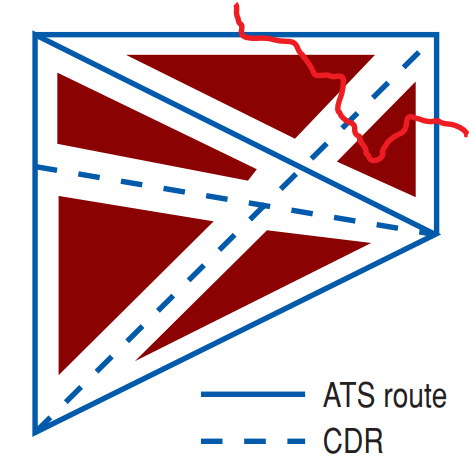
\includegraphics[width=0.25\linewidth]{figuras/estructura_cdr.png}
    \caption{Esquema de las rutas ATS convencionales y de las CDR.}
    \label{fig:estructura_cdr}
\end{figure}

\begin{figure}[H]
    \centering
    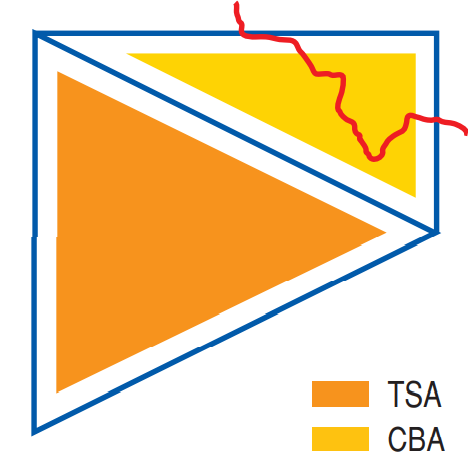
\includegraphics[width=0.25\linewidth]{figuras/estrutura_tsa_cba.png}
    \caption{Esquema de las áreas TRA, TSA y CBA.}
    \label{fig:estrutura_tsa_cba}
\end{figure}

\begin{figure}[H]
    \centering
    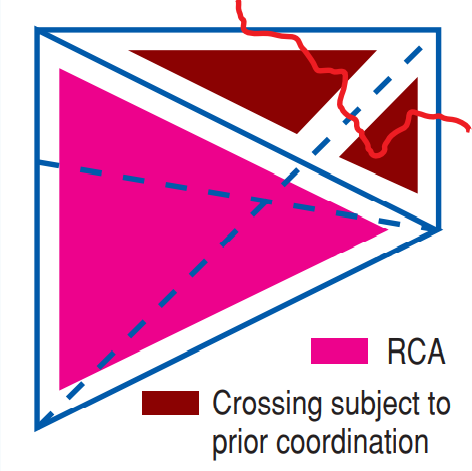
\includegraphics[width=0.25\linewidth]{figuras/estructura_rca.png}
    \caption{Esquema de las espacios aéreos PCA y RCA.}
    \label{fig:estructura_rca}
\end{figure}

\section{Entorno operativo del FUA}

Este sistema al operar en los Estados de la CEAC (Conferencia Europea de Aviación Civil) requiere que los Estados establezcan una coordinación civil y militar en tiempo real, que permita asignar estructuras flexibles de espacio aéreo diariamente. Para poner en marcha este sistema, se hará a través de los llamados “National Airspace Management Cells (ACMs)”, que se encargarán de asignar y promulgar la flexibilidad del espacio aéreo en base a la información que reciban tanto del entorno civil, como del militar.

Esta información a su vez la compartirán con el Network Manager (NM), cuyo cometido es difundir la disponibilidad diaria de las rutas ATS y la asignación diaria de los distintos espacios aéreos (restricciones, puntos intermedios obligatorios, etc). 

En la figura (\ref{fig:elementos_fua}) se puede observar el flujo de información descrito.

\begin{figure}[H]
    \centering
    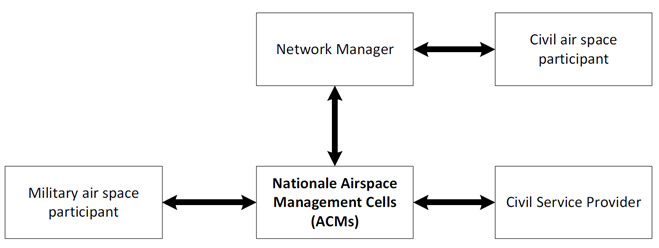
\includegraphics[width=1\linewidth]{figuras/elementos_fua.png}
    \caption{Elementos que constituyen el FUA.}
    \label{fig:elementos_fua}
\end{figure}

\section{Conclusiones y necesidad de un nuevo sistema}

Aunque como se ha comentado en la introducción de este apartado, la implementación del FUA ha sido desigual y no ha alcanzado todos los objetivos que se planteaban durante su periodo de definición, sí que se han observado algunas resultados positivos.

Entre estos aspectos positivos encontramos:

\begin{itemize}
    \item Se ha reducido la distancia, el tiempo y el combustible necesario para operar, mejorando la economía de los vuelos.
    \item Se ha incrementado la capacidad del sistema de control y se han reducido los retrasos.
    \item Se ha comprobado que funciona de manera más eficiente a la hora de separar operaciones civiles y militares.
    \item Ha permitido definir de manera más concreta las áreas de uso militar permitiendo que se adapten mejor a las necesidades de dichas operaciones.
\end{itemize}

Sin embargo, ya han aparecido nuevos proyectos que han hecho plantearse la necesidad de ir un paso más allá. En el horizonte aparece el AFUA, que realizará una revisión de lo conseguido hasta el momento, y buscará conseguir una coordinación aún mayor que permita aumentar aún más la capacidad y eficiencia del sistema de gestión del tránsito aéreo.

Durante la implantación del FUA, la integración del proceso de CDM mostró que aún existe un amplio margen de mejora. En particular, en la integración conjunta del \acrfull{asm}, \acrfull{atfcm} y el \acrfull{ats}, lo que permitirá disponer de más datos en tiempo real.

El propósito del sistema propuesto en este OCD, y que se comenzará a desarrollar a partir del apartado siguiente, será reemplazar las estructuras fijas por volúmenes de espacio aéreo con una configuración más dinámica, partiendo de la base de la cooperación civil–militar. Los avances que se consigan derivados de la implantación de este sistema darán como resultado la posibilidad de avanzar en otros sistemas como la \acrfull{dac}, el sistema Free Route y el \acrfull{swim}.

El conjunto integrado de todos estos sistemas permitirá dotar al espacio aéreo de una flexibilidad que será clave en un futuro en el que la demanda se haya incrementado notablemente.

\chapter{Sistema propuesto y esquema operativo}

Como se ha comentado en el apartado anterior, los resultados obtenidos de la implementación del \acrfull{fua} han sido dispares en el entorno europeo. Los niveles de aplicación que se han alcanzado dependen de la zona geográfica en la que nos encontremos.

Aunque sí es verdad que han aparecido consecuencias positivas de la implementación del FUA se consideran insuficientes, por lo que es necesario seguir buscando mejoras que permitan crear un sistema más sólido y con niveles de implantación regulares a lo largo del territorio europeo. Es en este contexto donde se comienza a definir el AFUA (Advanced Flexible Use of Airspace).
\section{Misión del sistema}

La implantación del AFUA tiene como objetivo proporcionar una mayor flexibilidad operativa a todos los usuarios del espacio aéreo mediante una configuración dinámica del mismo, que abarque todas las fases de la operación, desde la planificación inicial a la fase de análisis posterior a la operación, incluyendo la fase de ejecución.

Esta configuración dinámica nos permitirá reemplazar las distintas estructuras fijas utilizadas hasta ahora por volúmenes de espacio aéreo flexibles. Para conseguir esto, se debe tomar como piedra angular la coordinación civil–militar. Por lo que el primer objetivo del AFUA será conseguir que esta coordinación sea a través del ASM.

Los usuarios del espacio aéreo, civiles o militares, verán reflejada la implementación del AFUA de la siguiente manera:

\begin{itemize}
    \item \textbf{Militar.} La gestión dinámica del espacio aéreo permitirá una planificación y gestión de las operaciones militares mucho más cercana al periodo de operación en el caso de que sea necesario. La automatización proporcionada por las herramientas de soporte del ASM mejorará el proceso de decisión y aportará funcionalidades adicionales, como la capacidad de predicción de la situación a futuro, lo que mejorará la transparencia en las fases de ejecución y planificación.
    \item \textbf{Civil.} La gestión dinámica permitirá en este caso una mejorar planificación y gestión del balance necesario entre capacidad y demanda en los tres niveles de gestión.
\end{itemize}

En su objetivo de asegurar un uso óptimo del espacio aéreo disponible por todos los posibles usuarios, el AFUA hará imprescindible el desarrollo de un sistema de comunicaciones y apoyo en tiempo real. Este sistema permitirá mediante una continua actualización de una base de datos, con la información relativa a la fase de planificación y ejecución, que se establezca una coordinación directa entre los organismos locales de gestión civil y militar (AMC, ACC, etc) y el Network Manager.

De esta manera se mejorará la coordinación civil–militar y se tendrá un mayor conocimiento de la forma de operación de las distintas regiones de espacio aéreo. Además, esto permitirá aumentar la capacidad y reducir la carga de trabajo asociada a la fase de ejecución.

\subsection{Estructura organizacional del AFUA}

La estructura del AFUA, no es muy diferente de la del FUA, sino que utilizará herramientas y procedimientos más avanzados para lograr que el FUA proporcione estructuras del espacio aéreo más flexibles y eficientes. Por ello no se va a repetir la estructura ya expuesta en anteriores apartados sino que a continuación se van a exponer los cambios y mejoras respecto a ella. El AFUA introduce la siguiente serie de mejoras.

\subsubsection{Mejoras en la toma de decisiones}

Se realizará mediante \acrfull{cdm} que es el proceso mediante el cual todas las decisiones ATM, excepto las del ATC, se toman en base al intercambio de información relevante acerca de las operaciones entre los operadores civiles y militares.  

Mediante este proceso, la comunidad ATM comparte información necesaria para llevar a cabo las operaciones. Dicho intercambio de información posibilita la toma de decisiones, garantizando que las partes interesadas reciben información precisa y oportuna, esencial para la planificación de sus respectivas operaciones. Al permitir la toma de decisiones basada en información, se aumenta la previsibilidad en caso de eventos imprevistos o interrupciones, lo que permite hacer una utilización más óptima del espacio aéreo. El AFUA, pretende integrar la actividad del ATFCM, ASM y ATS utilizando el proceso de CDM, tal y como se muestra en la figura (\ref{fig:cdm}).

\begin{figure}[H]
    \centering
    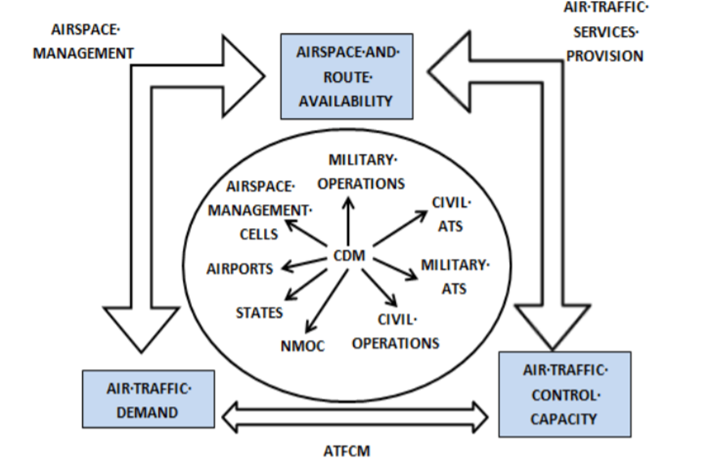
\includegraphics[width=1\linewidth]{figuras/cdm.png}
    \caption{Proceso CDM con las partes interesadas en el espacio aéreo.}
    \label{fig:cdm}
\end{figure}

\subsubsection{Trayectorias dinámicas y Free Routing}

Las operaciones de aeronaves civiles ya no se basarán en establecer un conjunto de rutas ATS fijas e invariables. El presente OCD introduce el concepto de trayectorias dinámicas que permitirán a las aeronaves, cambiar sus rutas en función de las actividades militares reservadas.  Los usuarios, sabrán en todo momento qué espacio aéreo está reservado para determinadas actividades. Dicha información les permitirá cambiar su ruta para evitar penetrar en dichos espacios aéreos. 

Este cambio se podrá realizar con la ayuda del concepto de Free Route, que permitirá a los usuarios del espacio aéreo tener más flexibilidad a la hora de elegir su trayectoria. 

\subsubsection{Mejoras en el intercambio de datos}

Para que todo lo mencionado anteriormente se pueda llevar a cabo de forma segura es necesario intercambiar gran cantidad de información entre lo operadores civiles y militares. Por esta razón es necesario disponer de un sistema capaz de ofrecer la información necesaria para que las operaciones se lleven a cabo de la manera más eficiente posible. Para ello es necesario el concepto de \acrfull{swim}, que será el sistema capaz de informar, notificar y dotar de más flexibilidad al sistema propuesto en el presente OCD.

\subsubsection{Uso de configuraciones de espacio aéreo}

El objetivo del AFUA, será reemplazar las estructuras fijas del espacio aéreo con volúmenes de espacio aéreo disponibles de forma dinámica. Este es uno de las evoluciones y cambios más grandes respecto el FUA. Las estructuras del FUA eran mucho más fijas y estáticas (ver apartado (\ref{tit:fua_estructura})) 

El AFUA utilizará las siguientes nuevas configuraciones:

\begin{enumerate}
    \item \textbf{Variable Profile Area (VPA)}
    
    Permite la asignación y gestión flexible de pequeños módulos fijos predefinidos de espacio aéreo. Su implementación permite una mejor respuesta a los requisitos y limitaciones militares y mejora la coordinación civil-militar, incluida la actualización del estado del espacio aéreo en tiempo real.

    \begin{figure}[H]
        \centering
        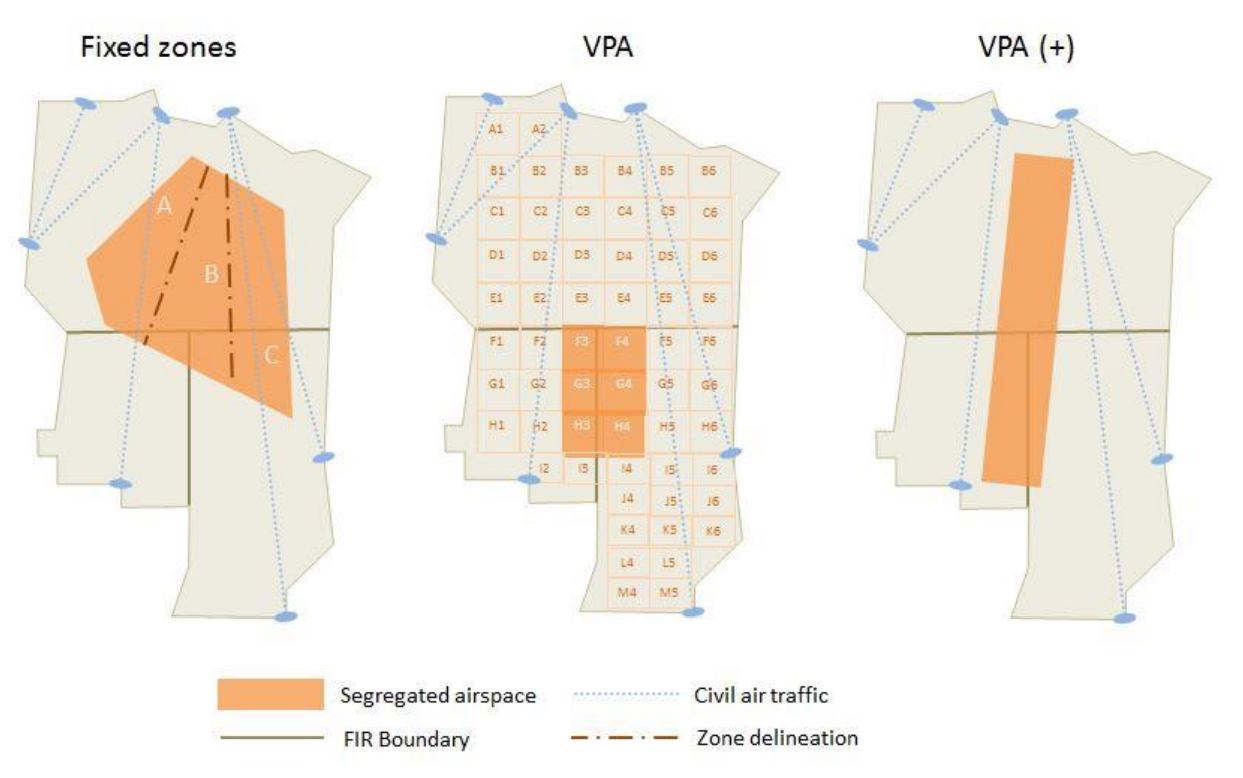
\includegraphics[width=1\linewidth]{figuras/vpa.png}
        \caption{Evolución de sectores fijos (FUA) a VPA (AFUA).}
        \label{fig:vpa}
    \end{figure}

    \item \textbf{Dynamic Mobile Area (DMA)}
    
    Son áreas destinadas al uso militar que permiten mejorar la flexibilidad del espacio aéreo. Se definen como un volumen de espacio aéreo en 4 dimensiones y se utiliza para proteger las actividades militares del tráfico civil. Existen tres tipos de DMAs:

    \begin{itemize}
        \item \textbf{Tipo 1:} son áreas definidas (dimensiones laterales y verticales) y asignadas (marco de tiempo de activación) para satisfacer las necesidades del usuario del espacio aéreo. La ubicación óptima del DMA se decide caso por caso. El AMC asignará un DMA en una ubicación específica para una misión determinada a fin de minimizar el impacto en el tráfico civil esperado.
        
        \begin{figure}[H]
            \centering
            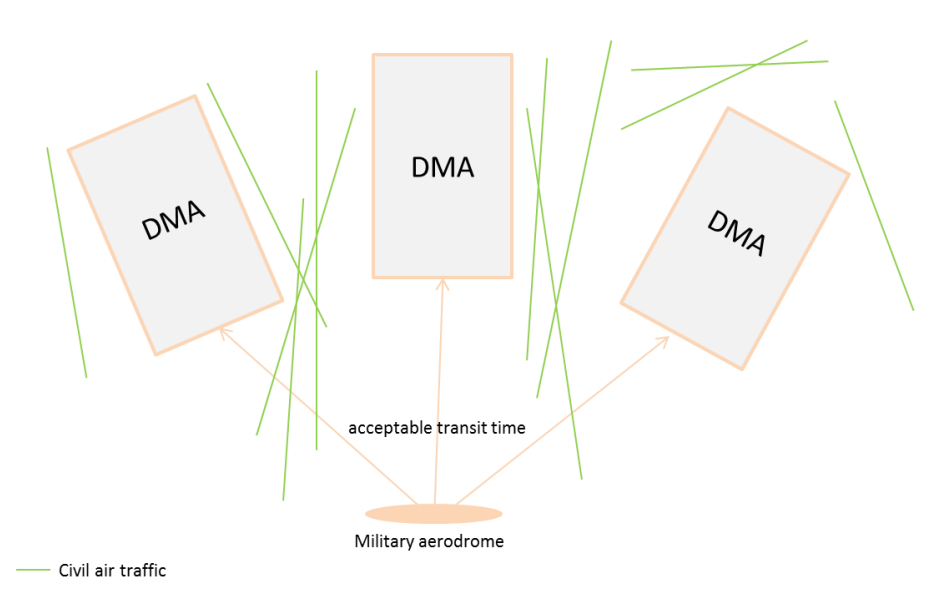
\includegraphics[width=0.8\linewidth]{figuras/dma_1.png}
            \caption{DMAs de tipo 1.}
            \label{fig:dma_1}
        \end{figure}
    
        \item \textbf{Tipo 2:} son áreas definidas con dimensiones laterales y verticales y asignación de tiempo de acuerdo con las necesidades del usuario del espacio aéreo. La diferencia con las DMAs del tipo 1 es que la ubicación del área cambiará a medida que ocurra la misión. Las misiones militares a menudo incluyen varias tareas en diferentes ubicaciones y diferentes niveles de vuelo (por ejemplo, reabastecimiento de combustible en el aire, ejercicios de combate, etc.). No siempre es posible asignar un área única que abarque todas estas tareas, ya que segregaría una parte importante del espacio aéreo y eso afectaría drásticamente los flujos de tráfico civil. 
        
        Los DMA de tipo 2 consisten en varias áreas más pequeñas definidas a lo largo de la trayectoria de la misión, que limitan el impacto en los flujos de tráfico civil y aseguran la asignación del espacio aéreo para los militares.
        
        \begin{figure}[H]
            \centering
            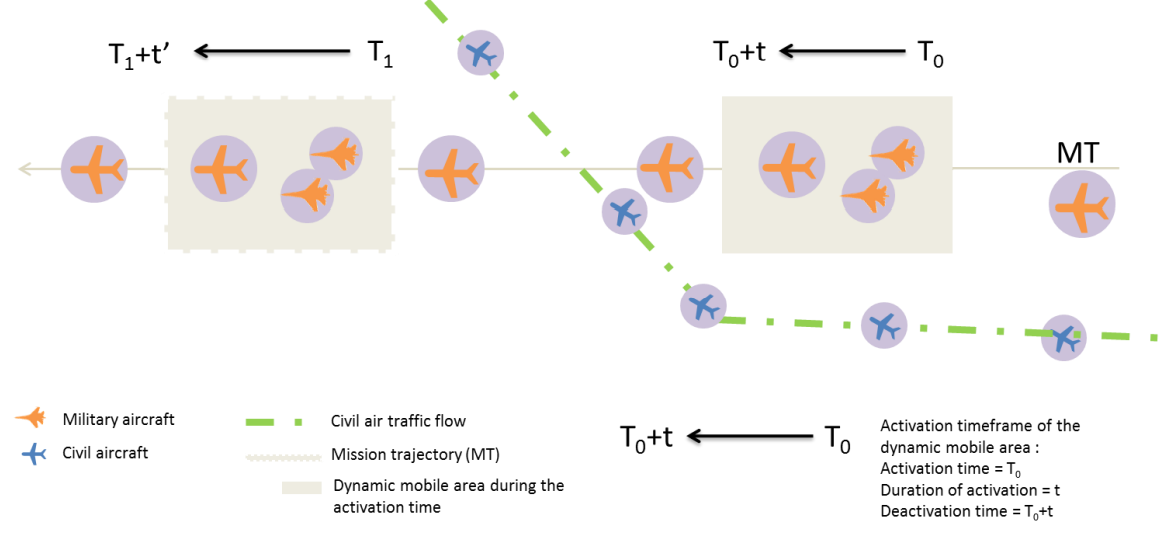
\includegraphics[width=0.8\linewidth]{figuras/dma_2.png}
            \caption{DMAs de tipo 2.}
            \label{fig:dma_2}
        \end{figure}
        
        \item \textbf{Tipo 3:} son áreas definidas con dimensiones laterales y verticales alrededor de actividades en movimiento que requieren una separación adecuada de las trayectorias de otros usuarios del espacio aéreo. Por lo tanto, los DMA de tipo 3 son burbujas que se mueven con el avión militar para separar el vuelo militar del resto del tráfico. Este tipo de DMA no solo minimiza la segregación del espacio aéreo, sino que también es beneficioso para el usuario del espacio aéreo militar al aumentar la flexibilidad. 
        
        \begin{figure}[H]
            \centering
            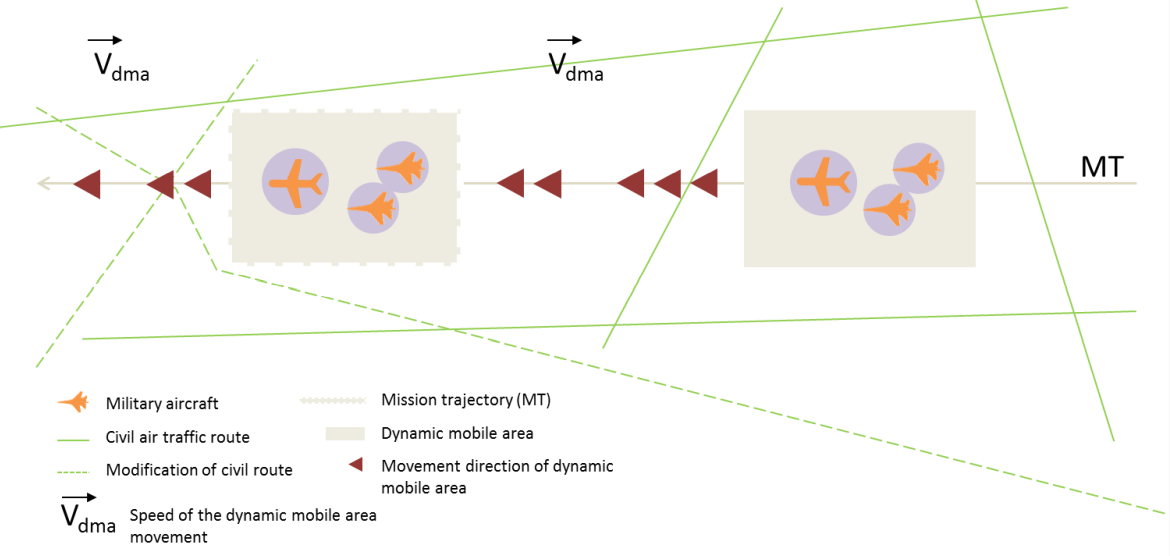
\includegraphics[width=0.8\linewidth]{figuras/dma_3.png}
            \caption{DMAs de tipo 3.}
            \label{fig:dma_3}
        \end{figure}
    \end{itemize}
\end{enumerate}

\subsection{Niveles de gestión. Estrategias}

Al igual que en el FUA, es necesario definir una serie de niveles que permitan gestionar las tareas relativas a la armonización y el conocimiento común de las medidas ASM/ATFCM y ATS.

En el caso del AFUA se distinguen 4 niveles como se puede ver en la figura (\ref{fig:niveles}):

\begin{figure}[H]
    \centering
    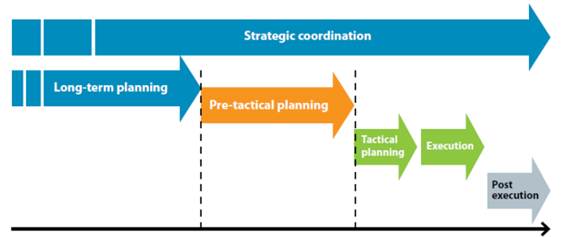
\includegraphics[width=1\linewidth]{figuras/niveles.png}
    \caption{Esquema de niveles de gestión y estrategias.}
    \label{fig:niveles}
\end{figure}

\subsubsection{Planificación estratégica}\label{tit:level1}

Comprende desde varios años antes de la operación hasta 7 días antes de la misma. La información relativa a las reservas de espacio aéreo orientadas a maniobras o ejercicios militares se conoce con antelación.

Se introducen un nuevo sistema que permite reservar regiones de espacio aéreo de manera provisional. Este sistema de reservas está específicamente diseñado para que dichas regiones de espacio aéreo puedan ser modificadas de acuerdo a las necesidades. 

\subsubsection{Fase pre-táctica}\label{tit:level2}

Comprende desde 7 días antes de la operación hasta el día de la misma. 
La información que se utiliza en esta fase para la planificación del espacio aéreo en los días posteriores está relacionada con los AUP’s (Airspace Use Plan) y UUP’s (Updated Airspace Use Plan) tanto a nivel nacional, como de bloque funcional (FAB’s) y del conjunto europeo de la red (EAUP y EUUP).

Además, contiene todas la actualizaciones necesarias acerca de la disponibilidad esperada de los CDR’s (Coded Departure Routes) y las reservas de espacio aéreo en el día de la operación.

\subsubsection{Fase táctica}\label{tit:level3}

Es la correspondiente al día de la operación.
La información utilizada es la relativa a la planificación a corto plazo y a la utilización del espacio aéreo en tiempo real.

Se define el status de las diferentes zonas de espacio aéreo como disponible, reservado, en uso o liberado. Proporciona información acerca de la forma y localización real de las porciones consideradas de espacio aéreo. 

Confirma lo definido en la fase pre-táctica relativo a la disponibilidad de los CDR’s y las reservas de espacio aéreo.

\subsubsection{Fase posterior a la operación}

Es una novedad respecto a lo planteado en el FUA. Tiene lugar el día posterior a la operación.
En esta fase la información está relacionada con las reservas y la utilización real que se dio a dichos espacios aéreos.

\subsection{Geografía y ubicación de las operaciones}

En el sistema AFUA que se pretende implantar en el espacio aéreo europeo, es clave la definición del proyecto del Cielo Único Europeo.

Dentro de la regulación asociada a este proyecto se hace hincapié en que todos los Estados miembros deben introducir todas las medidas necesaria para asegurar la implementación de los denominados bloques funcionales o \acrfull{fab}, que jugarán un papel clave en la implementación del AFUA.

Estos FAB, constituyen unos bloques de espacio aéreo basada en requisitos operacionales y establecidos sin tener en cuenta las fronteras entre Estados. En ellos, la provisión de servicios de navegación aérea y todas las funciones asociadas, están enfocados hacia la optimización de las actuaciones. 

En total, se han definido 9 iniciativas de bloques funcionales, como aparecen identificados en la figura (\ref{fig:fab}).

La introducción de estos bloques funcionales es clave en el desarrollo del AFUA, puesto que al eliminarse las fronteras nacionales, será más sencillo dirigir la definición de los espacios aéreos correspondientes con unas operaciones más optimizadas. 

El hecho de que los proveedores de navegación aérea trabajen de manera conjunta, permitirá flexibilizar los usos que se da al espacio aéreo en un marco de colaboración común.

\begin{figure}[H]
    \centering
    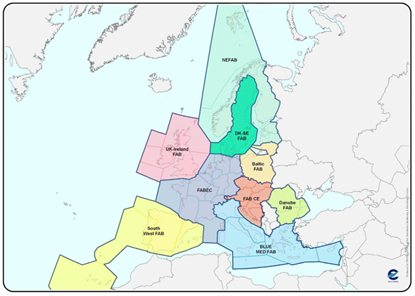
\includegraphics[width=0.8\linewidth]{figuras/fab.png}
    \caption{Bloques funcionales en Europa.}
    \label{fig:fab}
\end{figure}

Los objetivos que se marcan a la hora de definir los bloques funcionales son los siguientes:

\begin{itemize}
    \item Incrementar la seguridad.
    \item Aumentar la capacidad.
    \item Balancear los costes mediante una estructura más efectiva de rutas y provisión de servicios ATC.
    \item Conseguir una mayor eficiencia en las operaciones.
    \item Reducir el impacto sobre el entorno.
    \item Incrementar la efectividad de las operaciones militares.
\end{itemize}

En cuanto a su aplicación vertical, el AFUA se implementará en el espacio aéreo superior, es decir, por encima del FL195. La justificación de su implementación en el espacio aéreo superior viene dada por el hecho de que la coordinación de la parte civil y militar proporcionará más beneficios en los niveles de ruta de las aeronaves.

No hay que olvidarse de que el objetivo principal del sistema propuesto es evitar cambios de rutas debido a la segregación del espacio aéreo civil y militar. Esos cambios de trayectoria tendrán como resultado rutas más largas que llevan a incrementar el consumo de combustible en las aeronaves civiles y por tanto repercutirán de manera negativa en los costes y en el medioambiente. Por tanto, la aplicación del AFUA en esos niveles resulta indispensable para solucionar los problemas derivados de la segregación del espacio aéreo superior y proporcionar más flexibilidad dentro del mismo.

\begin{figure}[H]
    \centering
    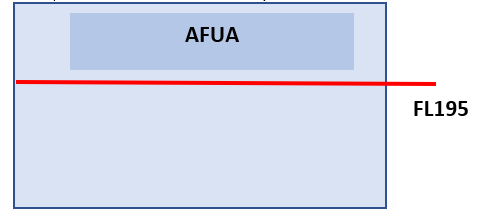
\includegraphics[width=0.8\linewidth]{figuras/afua_vertical.png}
    \caption{Aplicabilidad vertical del AFUA.}
    \label{fig:afua_vertical}
\end{figure}

\subsection{Sistemas relacionados}

A lo largo de este OCD ya han surgiendo varios sistemas que no solo están relacionados con el AFUA sino que son cruciales para que el concepto se pueda implementar y se convierta en un sistema real. En este apartado se van a listar dichos sistemas y hacer un pequeño resumen de ellos.

\subsubsection{System Wide Information Management (SWIM)}

El \acrfull{swim} son las normas, infraestructura y gobernanza que permiten la gestión de la información relacionada con el ATM y su intercambio entre partes cualificadas a través de servicios interoperables.

Dentro de SESAR se definen los siguientes principios clave  para el SWIM:

\begin{itemize}
    \item La información debe compartirse de forma segura en todo el sistema.
    \item La información pertinente estará disponible cuando y donde se necesite.
    \item La información se podrá personalizar, filtrar y acceder a ella, según sea necesario.
    \item El sistema incluirá todos los medidas de ciberseguridad necesarias para asegurar la confidencialidad, la integridad, la disponibilidad y la protección de los datos, las redes y los sistemas de control, la continuidad de las operaciones y las comunicaciones interoperables seguras.
    \item Autenticación para el acceso de los usuarios.
    \item La calidad inicial de la información será responsabilidad del emisor, la manipulación posterior no comprometerá su calidad.
    \item El intercambio de información puede ajustarse para mitigar cualquier problema de propiedad.
    \item La gestión de la información utilizará atributos de información armonizados a nivel mundial.
\end{itemize}

\subsubsection{Colaborative Decision Making (CDM)}

El \acrfull{cdm} es un proceso que sirve para apoyar otras actividades. Puede aplicarse a lo largo de la línea de tiempo de las actividades, desde la planificación estratégica (por ejemplo, las inversiones en infraestructuras) hasta las operaciones en tiempo real. El CDM no es un objetivo, sino una forma de alcanzar los objetivos de rendimiento de los procesos que apoya. Se espera que estos objetivos de rendimiento se acuerden en colaboración. 

Dado que la aplicación del CDM requerirá probablemente inversiones, éstas deberán justificarse de acuerdo con el enfoque basado en el rendimiento.

Aunque el intercambio de información es un factor importante, esto no es suficiente para realizar el CDM y sus objetivos. El CDM también requiere procedimientos y reglas predefinidos y acordados para garantizar que las decisiones de colaboración se tomen de forma rápida y equitativa.

El CDM garantiza que las decisiones se tomen de forma transparente, basándose en la mejor información disponible proporcionada por los participantes de forma oportuna y precisa.

El proceso para implementar el CDM en el AFUA o en cualquier otro sistema tiene las siguientes fases:

\begin{enumerate}
    \item Identificación de la necesidad del CDM.
    \item Análisis del CDM.
    \item Especificación y verificación del CDM.
    \item Caso de rendimiento del CDM.
    \item Validación y aplicación del CDM.
    \item Funcionamiento, mantenimiento y mejora del CDM. Esto es un proceso continuo.
\end{enumerate}

Es importante que los resultados de todas estas fases se compartan entre los miembros de la comunidad involucrados.

\subsubsection{Dynamic Airspace Configuration (DAC)}

\acrfull{dac} es un nuevo paradigma operativo que propone migrar del actual espacio aéreo estructurado y estático a un espacio aéreo dinámico capaz de adaptarse a la demanda de los usuarios al tiempo que satisface las cambiantes limitaciones de la meteorología, la congestión del tráfico y la complejidad, así como una flota de aviones muy diversa.

El DAC se ocupa de tres componentes principales: 

\begin{enumerate}
    \item La organización global del espacio aéreo.
    \item El cambio dinámico del espacio aéreo para satisfacer la demanda.
    \item Una caracterización genérica del espacio aéreo.
\end{enumerate}

El primer componente se refiere a la organización estratégica del espacio aéreo y a la creación de nuevas clases de espacio aéreo para aprovechar los conceptos y tecnologías que se espera que estén disponibles para 2025. 

El segundo componente se refiere a la reconfiguración dinámica del espacio aéreo necesaria para acomodar una demanda fluctuante. 

El tercer componente se refiere a los diseños "genéricos" del espacio aéreo que podrían promover la intercambiabilidad entre las instalaciones y los controladores mediante la eliminación de los componentes estructurales y funcionales del espacio aéreo que requerirían una formación específica del mismo.

\subsubsection{Free Route Airspace (FRA)}

\acrfull{fra} es un espacio aéreo especificado dentro del cual los usuarios pueden planificar libremente una ruta entre un punto de entrada y un punto de salida definidos. En función de la disponibilidad del espacio aéreo, la ruta puede planificarse directamente de uno a otro o a través de puntos de paso intermedios (publicados o no), sin referencia a la red de rutas ATS. Dentro de este espacio aéreo, los vuelos siguen estando sujetos al control del tráfico aéreo.

En un FRA el operador puede elegir su ruta con sólo algunas limitaciones (por ejemplo, puntos fijos de entrada y salida y la necesidad de evitar zonas de peligro, TRA o TSA), a diferencia de la situación en la que deben utilizarse las vías aéreas estándar. En la mayoría de los casos se elegirá la línea recta entre un punto de entrada y un punto de salida. 

Si por alguna razón esto no es apropiado (por ejemplo, hay que evitar una zona de peligro) se pueden especificar puntos de giro adicionales. Estos pueden ser ayudas a la navegación, puntos de navegación publicados o puntos con coordenadas especificadas.

La introducción de la FRA en Europa es un proceso gradual. La mayoría de los estados han decidido empezar con una implementación limitada (por ejemplo, durante las horas nocturnas) y luego ampliarla gradualmente.

A finales de 2020, 46 ACC habían implementado la FRA al menos parcialmente (pero en su mayoría sobre la base de H24). Además, hay muchas implementaciones transfronterizas, es decir, más de una ACC que participa en una iniciativa de FRA.
\section{Políticas y restricciones operativas}

\subsection{Principios para la implementación del AFUA}

Las políticas y principios que rigen la implementación del concepto \acrfull{afua} en el espacio aéreo europeo están desarrollados en el \citetitle{CE2150/2005} \cite{CE2150/2005}. 

La utilización flexible del espacio aéreo es un concepto de gestión del espacio aéreo, descrito por la \acrfull{oaci} y desarrollado por la \acrfull{eurocontrol}, según el cual el espacio aéreo no debe designarse como espacio aéreo puramente civil o militar, sino como un continuum en el que deben satisfacerse las necesidades de todos los usuarios en la mayor medida posible.  Eurocontrol ha recibido el mandato de asistir a la Comisión en el desarrollo de normas de aplicación de la utilización flexible del espacio aéreo. 

El concepto de \acrfull{afua} se ajustará a los siguientes principios:

\begin{itemize}
    \item La coordinación entre las autoridades civiles y militares se organizará a nivel estratégico, pretáctico y táctico mediante el establecimiento de acuerdos y procedimientos encaminados a aumentar la seguridad y la capacidad del espacio aéreo y a mejorar la eficacia y flexibilidad de las operaciones aéreas.
    
    \item Se deberá establecer y mantener la coherencia entre la gestión del espacio aéreo, la gestión de la afluencia del tránsito aéreo y las funciones de los servicios de tránsito aéreo con el fin de asegurar una eficiente planificación, distribución y utilización a todos los usuarios en los tres niveles de gestión del espacio aéreo.
    
    \item La reserva de espacio aéreo para uso exclusivo o específico de determinadas categorías de usuarios tendrá carácter temporal, se aplicará sólo durante períodos de tiempo limitados en función de la utilización real y se prescindirá de ella en cuanto cese la actividad que la haya motivado.
    
    \item Los Estados miembros cooperarán entre sí para la aplicación eficiente y coherente del concepto de utilización flexible del espacio aéreo a través de las fronteras nacionales o los límites de las regiones de información de vuelos y, en particular para atender las actividades transfronterizas. La cooperación abarcará todos los aspectos jurídicos, operativos y técnicos pertinentes.
    
    \item Las dependencias y usuarios de servicios de tránsito aéreo harán el mejor uso posible del espacio aéreo disponible.
\end{itemize}

\subsection{Uso y aplicabilidad}

Como se ha mencionado anteriormente la coordinación entre las autoridades civiles y militares se organizarán en tres niveles: estratégico, práctico y táctico. Para que las operaciones puedan llevarse a cabo en estos tres niveles, es necesario definir un conjunto de políticas y normas que deberán aplicarse en cada fase para aumentar la seguridad, eficacia y flexibilidad de las operaciones aéreas.

\subsubsection{Nivel estratégico}

Los Estados miembros desempeñarán las siguientes funciones:

\begin{enumerate}
    \item Revisar con regularidad las necesidades de los usuarios, especialmente en el entorno militar. Esto contribuirá a ajustar la demanda a la capacidad del espacio aéreo y evitará los problemas en el nivel táctico.
    \item Validar las actividades que precisen de reserva o restricciones del espacio aéreo. En esta parte, la contribución del factor humano resulta imprescindible, pues será el responsable de realizar dichas validaciones.
    \item Definir estructuras temporales del espacio aéreo y procedimientos que ofrezcan opciones múltiples de reserva y rutas. Según se ha definido en apartados anteriores, será necesario hacer uso de espacio aéreos militares dinámicos. En función de la eficiencia de estos espacios se habían definido tres niveles, por tanto, la función del factor humano será determinar qué tipo de estructura es la más adecuada para el tipo de operación que va a tener lugar.
    \item Establecer criterios y procedimientos que permitan la creación y el uso de límites laterales y verticales ajustables del espacio aéreo necesario para acoger diversas variaciones de trayectorias de vuelo y cambios a corto plazo en los vuelos.
    \item Evaluar las estructuras del espacio aéreo nacional y la red de rutas con el fin de planificar estructuras y procedimientos flexibles del espacio aéreo.
    \item Determinar las condiciones específicas en las que la responsabilidad de la separación de los vuelos civiles y militares recaerá en las dependencias civiles y militares de servicios de tránsito aéreo o en las dependencias militares de control. Será el controlador el encargado de controlar que las mínimas de separación entre aeronaves civiles y militares se cumplen. 
    \item Desarrollar un uso transfronterizo del espacio aéreo con los Estados miembros cuando así lo dicten la afluencia del tránsito y las actividades de los usuarios. Para ello será necesario que todos los operadores del espacio aéreo compartan un conjunto de reglas técnicas y operacionales comunes. Sobrepasar los límites de las fronteras, ayudará a flexibilizar más el espacio aéreo, así como poder ofrecer soluciones más eficientes.
    \item Coordinar la política de gestión del espacio aéreo con la de los Estados miembros para abordar de manera conjunta la utilización del espacio aéreo a través de las fronteras nacionales y los límites de las regiones de información de vuelos.
    \item Establecer y ofrecer a los usuarios estructuras de espacio aéreo en estrecha cooperación y coordinación con los Estados miembros cuando las estructuras de espacio aéreo correspondientes tengan importantes repercusiones en el tránsito transfronterizo o en los límites de las regiones de información de vuelos con vistas a asegurar una utilización óptima del espacio aéreo a todos los usuarios de la Comunidad.
    \item Establecer con los Estados miembros un conjunto de normas comunes para la separación entre los vuelos civiles y militares en las actividades transfronterizas.
    \item Establecer mecanismos de consulta entre las personas u organismos contemplados en el apartado 3 y todas las partes y organizaciones interesadas para satisfacer debidamente las necesidades de los usuarios.
    \item Evaluar y revisar los procedimientos y el funcionamiento de las operaciones dentro de la utilización flexible del espacio aéreo.
    \item Establecer mecanismos para almacenar los datos de las solicitudes, asignación y utilización real del espacio aéreo para su posterior análisis y para la planificación de actividades.
    \item En aquellos Estados miembros en los que tanto las autoridades civiles y como las militares compartan la responsabilidad o participen en la gestión del espacio aéreo, las funciones anteriores se realizarán a través de un proceso conjunto civil-militar.
    \item Los Estados miembros identificarán a las personas y organismos responsables de asumir las funciones enumeradas en los apartados anteriores y los comunicarán a la Comisión. La Comisión mantendrá la lista de dichas personas y organismos y la publicará a fin de facilitar la cooperación entre los Estados miembros.
\end{enumerate}

\subsubsection{Nivel pretáctico}

Para este nivel se han definido las siguientes actuaciones para los Estados miembros:

\begin{enumerate}
    \item De acuerdo con lo que se ha definido en el punto 1 de la fase estratégica, los Estados miembros deben nombrar una célula de gestión encargada de asignar el espacio aéreo para cumplir con las condiciones y procedimientos definidos respecto a la revisión continua de las necesidades de los usuarios del espacio aéreo. En aquellos Estados, en los que la responsabilidad de la gestión del espacio aéreo 	recaiga sobre autoridades tanto civiles como militares, la célula que se forme debe 	adoptar un carácter conjunto civil y militar.
    
    \item Dos o más Estados miembros podrán establecer una célula conjunta de gestión del espacio aéreo. Es interesante sobre todo en zonas fronterizas, de cara a coordinar mejor las 		operaciones. Estas células tendrán como objetivo responder de una manera más 	adecuada a la demanda, centrándose en la optimización de las operaciones.

    \item Los Estados miembros deben proveer a las células de gestión de espacio aéreo con los sistemas de apoyo adecuados. Es imprescindible garantizar que serán capaces de gestionar las operaciones de asignación de espacio aéreo, así como de comunicar la disponibilidad del mismo a los distintos usuarios afectados, a otras células de gestión de espacio aéreo, a los proveedores de servicios de tránsito aéreo y a todo aquel que pueda requerir dicha información.
\end{enumerate}

\subsubsection{Nivel táctico}

Dentro del nivel táctico las actuaciones de los Estados miembros serán las siguientes:

\begin{enumerate}
    \item Deben garantizar que se crearán los procedimientos necesarios para asegurar una correcta coordinación civil y militar. También se debe asegurar una comunicación efectiva entre las dependencias de servicios de tránsito aéreo y aquellas dependencias militares de control, de manera que se permita el intercambio de información y datos acerca del espacio aéreo, para asegurar una correcta activación, desactivación o redistribución en tiempo real de los distintos espacios aéreos asignados durante el nivel pretáctico.
    
    \item Los Estados miembros deben velar porque las dependencias militares de control y las dependencias de servicios de tránsito aéreo se comuniquen mutuamente todos los cambios que puedan ocurrir durante la activación planificada del espacio aéreo. Esta comunicación debe realizarse de manera eficiente para notificar los posibles cambios a todos los usuarios afectados por la situación del espacio aéreo.
    
    \item Se debe garantizar que se introducirán los procedimientos de coordinación necesarios, así como medios de apoyo a las operaciones entre dependencias militares y dependencias de servicios de tránsito aéreo. Se debe asegurar que la gestión de la interacción de vuelos civiles y militares es absolutamente segura.
    
    \item Los Estados miembros velarán por el establecimiento de procedimientos de coordinación entre dependencias civiles y militares de servicios de tránsito aéreo, que permitan una comunicación directa de la información. Esta información está centrada en la resolución de situaciones concretas de tránsito dentro de un mismo volumen de espacio aéreo en el que estén prestando servicios tanto controladores civiles como militares.
    
    La información pertinente, se pondrá a disposición cuando sea necesario por razones de seguridad, mediante un rápido intercambio de datos de vuelo, entre los que se incluirá la posición e intención de vuelo de las aeronaves. Los destinatarios de dicha información pueden ser tanto controladores civiles, como militares.
    
    \item En el caso de operaciones transfronterizas, los Estados miembros deben garantizar que las dependencias civiles de servicios de tránsito aéreo y las dependencias militares (implicadas directamente en la provisión de servicios de tránsito aéreo o afectadas por dichas operaciones) llegan a un acuerdo de procedimientos comunes para la gestión de situaciones específicas del tránsito y para mejorar la gestión en tiempo real del espacio aéreo.
\end{enumerate}

\subsection{Restricciones operacionales}

A pesar de la desaparición de las fronteras terrestres, las fronteras en el espacio aéreos siguen estando presentes. Por esta razón, la Comisión Europea, adoptó el 10 de octubre de 2001, un conjunto de medidas con el objetivo de establecer el Cielo Único Europeo para finales del 2004. El objetivo es poner fin a la fragmentación del espacio aéreo en la Unión Europea, creando un espacio aéreo eficiente y sin fronteras. Las siguientes razones dificultan la puesta en marcha de este concepto, limitando su uso.  

Los estados miembros deben cooperar de forma eficiente para poder desarrollar este concepto. Esta cooperación entre las diferentes FIR debe acentuarse en las fronteras de los diferentes estados mediante la definición de una base técnica, operacional y legal común. La dificultad de esta coordinación en las fronteras entre estados es una de las mayores limitaciones del proyecto.

Por el lado militar, existen múltiples limitaciones, las cuales pueden agruparse en cinco bloques:

\begin{enumerate}
    \item \textbf{Limitaciones económicas:} las limitaciones presupuestarias, como consecuencia de la actividad militar sin ánimo de lucro, pueden dificultar la implementación de nuevos equipos en aviones militares a pesar de la creciente necesidad de evolucionar junto con nuevas iniciativas de ATM. Para dar solución a este problema, cada Estado, deberá subvencionar económicamente la puesta en marcha de este sistema debido a que, como se ha comentado en apartados anteriores, su implantación acarrea numerosos beneficios operacionales, medioambientales y económicos. 
    
    \item \textbf{Limitaciones operacionales:} : muchas de las operaciones militares son únicas y requieren una atención especial para llevarse a cabo. Por ejemplo, operaciones como vigilancia o patrullaje aéreo o extinción de incendios exigen la máxima prioridad y no pueden adaptarse a ninguna demora o denegación de acceso a un determinado espacio aéreo. Por ello, es necesario que el factor humano catalogue la importancia de las actividades militares que van a tener lugar y priorizar el uso del espacio aéreo en función de la importancia de las mimas.
    
    Una limitación operativa adicional viene impuesta por el artículo 3 del Convenio de Chicago, que prohíbe la operación de aeronaves estatales de un Estado sobre el territorio soberano de otro Estado sin autorización. Esta autorización puede incluir restricciones sobre cómo y dónde pueden operar dichas aeronaves. En consecuencia, las aeronaves de Estado no podrán aceptar autorizaciones ATC que modifiquen su ruta y/o altitud planificada de vuelo mientras se encuentren en el espacio aéreo soberano de otro Estado o que les hagan infringir el espacio aéreo. Por este motivo, los Estados deberán cooperar para uniformizar los modos de operación de las aeronaves militares con el fin de establecer una base común que permita cruzar fronteras libremente. 

    \item \textbf{Limitaciones técnicas:} constituye la mayor restricción para la implantación de este sistema debido a que los sistemas utilizados en las aeronaves militares difieren ligeramente de los usados en la aviación civil. Podemos encontrar diferencias en los siguientes sistemas de comunicación, navegación y vigilancia. La interoperabilidad entre los diferentes sistemas militares y civiles se discutirá en mayor detalle en los apartados siguientes. Para dar solución a este problema, cuando no pueda lograrse la interoperabilidad técnica, es decir, confiar en la capacidad de intercambio de información entre equipos o sistemas, la aplicación de procedimientos adicionales puede ser una opción alternativa para lograr el nivel de seguridad requerido y dar cabida a las aeronaves militares en el espacio aéreo en el que se admiten operaciones mixtas (civiles y militares).
    
    \item \textbf{Limitaciones en el intercambio de información:} las operaciones militares suelen estar protegidas y se evita compartir información excesiva con el exterior por motivos de seguridad (operaciones especiales, ensayos militares,etc.).  Por tanto, este aspecto restringe el intercambio de información entre los distintos participantes del espacio aéreo. 
    
    \item \textbf{Limitaciones en los procesos de certificación:} durante las últimas décadas, la evolución de la tecnología ha llevado a un aumento de los requisitos de las aeronaves cuando operan en cierto espacio aéreo (por ejemplo, RVSM, ADS-B); la evolución hacia operaciones basadas en trayectorias se sumará al aumento de los requisitos de las aeronaves. Las aeronaves militares que no pueden cumplir con los requisitos de equipamiento o certificación han buscado históricamente exenciones para operar en espacios aéreos con tales requisitos. Se espera que otorgar exenciones se vuelva más complejo en el futuro, ya que el número de requisitos y, por lo tanto, las exenciones necesarias, puede conducir a la imposibilidad (o con alta dificultad e impacto en el sistema) para compartir el mismo espacio aéreo. Por tanto, un mayor cumplimiento de las normas civiles facilitará el acceso al espacio aéreo de las aeronaves militares cuando se impongan requisitos específicos. La solución de este problema pasará por la sustitución y adopción por parte del entorno militar de los sistemas utilizados en la aviación civil.
\end{enumerate}
\section{Entorno Operativo}

\subsection{Sistema de navegación}

\subsubsection{Perfomance Based Navigation (PBN)}

El \acrfull{pbn} es un nuevo concepto basado en el uso de los sistemas de navegación de área (RNAV). 

La navegación basada en el desempeño según OACI, hace necesario que los sistemas de desempeño requeridos en navegación (RNP) y navegación de área (RNAV) sean definidos según los términos de precisión, integridad, disposición, continuidad y funcionalidad requeridos para las operaciones propuesta en el contexto de un espacio aéreo particular, cuando está respaldado por una infraestructura de navegación apropiada (GNSS u otro tipo de infraestructura aplicable a la navegación).

El concepto PBN, incluyendo el uso de señales obtenidas de satélites para las actuaciones en ruta y aproximación, está reemplazando gradualmente al sistema tradicional de navegación apoyada en ayudas terrestres a la navegación.

El concepto de PBN está compuesto de tres partes:

\begin{enumerate}
    \item Las especificaciones de navegación. Describen los requisitos de desempeño en términos de precisión, integridad y continuidad de las operaciones propuestas en un determinado espacio aéreo. También describe cómo se van a alcanzar estos requisitos. Deben llevar asociado unos apropiados estándares de conocimiento por parte de los pilotos, así como formación adecuada.
    
    \item La infraestructura de ayudas a la navegación que se utilizarán para cumplir con las especificaciones de navegación. La disponibilidad de esta infraestructura de ayuda tiene que ser tenida en cuenta a la hora de habilitar la aplicabilidad de este tipo de navegación.
    
    \item La aplicación a la navegación está referida a las especificación y ayudas a la navegación en el contexto de un espacio aéreo con rutas ATS y procedimientos de vuelo por instrumentos.
\end{enumerate}

Los beneficios asociados a la implantación del concepto PBN son los siguientes:

\begin{itemize}
    \item Reduce la necesidad de mantener una serie de ayudas específicas para la navegación y ruta y los costes asociados del uso y mantenimiento de estas.
    \item Evita la necesidad de desarrollar ayudas específicas para las operaciones con cada nueva evolución de los sistemas de navegación, lo que supone un coste demasiado elevado.
    \item Permite usar el espacio aéreo con una mayor eficiencia.
\end{itemize}

\subsubsection{Global Navigation Satellite System (GNSS)}

El \acrfull{gnss} transmite rangos de señales que se utilizan para el posicionamiento y localización de cualquier parte del globo terrestre. Estos satélites permiten determinar coordenadas geográficas y altitud en un punto dado.

El origen de este sistema es militar. La navegación por satélite permitía alcanzar valores de precisión que no se habían conseguido obtener con anterioridad, esto permitía aumentar la precisión sobre objetivos militar, aumentando la efectividad y reduciendo daños no deseados.

En el ámbito civil, los sistemas de posicionamiento por satélite son reconocidos como un elemento clave en los sistemas de comunicación, navegación y vigilancia (CNS). 

El GNSS comprende a todos los sistemas de navegación por satélite, los que ya han sido implementados (GPS y GLONASS) y los que están en desarrollo (GALILEO). Permiten la utilización de las redes de satélite como soporte a la navegación, ofreciendo una localización precisa de las aeronaves.

Cuando se encuentre plenamente desarrollado se prevé que pueda ser utilizado, en todas las fases de la operación de una aeronave, sin requerir ayuda de cualquier otro sistema de navegación convencional

\subsubsection{Instrumental Landing System (ILS) y Microwave Landing System (MLS)}

El \acrfull{ils} es el sistema de ayuda a la aproximación y aterrizaje establecido por OACI. Este sistema permite que un avión sea guiado con presión durante la aproximación a la pista, y en algunos casos, a lo largo de la misma.

El ILS está formado por dos subsistemas independientes, uno permite proporcionar guiado lateral, y el otro proporciona guía vertical. Se trata del localizador y la senda de planeo respectivamente.

El tipo de operaciones que permite el uso del ILS son las siguientes:

\begin{itemize}
    \item \textbf{Categoría I:} Altura de decisión no inferior a 60 m (200 ft) y con una visibilidad de no menos de 800 m o con un alcance visual en la pista no inferior a 550 m.
    \item \textbf{Categoría II:} Altura de decisión inferior a 60 m (200 ft) pero no inferior a 30 m (100 ft) y con un alcance visual en la pista no inferior a 300 m.
    \item \textbf{Categoría III:}
    \begin{itemize}
        \item \textbf{Categoría IIIA:} Altura de decisión inferior a 30 m (100 ft), o sin altura de decisión y un alcance visual en la pista no inferior a 175 m.
        \item \textbf{Categoría IIIB:} Altura de decisión inferior a 15 m (50 ft), o sin altura de decisión, y un alcance visual en la pista inferior a 175 m pero no inferior a 50 m.
        \item \textbf{Categoría IIIC:} Sin altura de decisión y sin restricciones de alcance visual en la pista.
    \end{itemize}
\end{itemize}

Por su parte, el MLS, es un sistema de ayuda al aterrizaje desarrollado por el servicio militar de EEUU, cuya principal misión es paliar una de las mayores limitaciones del sistema ILS. Trata de solucionar los problemas ocasionados por la presencia de irregularidades en el terreno y las distorsiones ocasionales.

Algunas de las ventajas proporcionadas por el MLS son las siguientes:

\begin{itemize}
    \item Equipamiento más preciso.
    \item Permite múltiples curvas de aproximación, a diferencia de la rigidez de la aproximación lineal del ILS.
    \item Es más barato.
\end{itemize}

Ambos sistemas serán sustituidos en el futuro por sistemas de navegación por satélite basados en GNSS, que son mucho más precisos que ambos.

\subsection{Entorno geopolítico}

La propia existencia del nacimiento del concepto \acrfull{fua} y su evolución en el concepto \acrfull{afua} es debido al contexto geopolítico en el que nace, Europa. En la otra zona del mundo que más se ha desarrollado la aviación, EEUU, este concepto no es tan necesario ya que todo el espacio aéreo pertenece al mismo país, el cual tiene un tamaño enorme. 

En cambio en Europa se tiene un espacio aéreo muy congestionado el cual está dividido por muchos estados. Los estados de la Unión Europea tienen un tamaño menos respecto a los presentes en otras zonas del mundo. En poco territorio se concentran muchos estados y cada uno tiene su ejercito y su soberanía respecto a su cielo. Esto hace que surjan los problemas derivados de las fronteras entre cada estado y que un vuelo pase por varios países cada uno con sus áreas restringidas para uso militar.

Es lógico que el concepto FUA haya surgido y tenido un mayor desarrolla en Europa, ya que es una zona con una problemática característica que el AFUA intenta solucionar.

\subsection{Instituciones}

El concepto del AFUA no es una idea abstracta que está en el aire sino que es un concepto creado, desarrollado y sustentado por un contexto social y unas instituciones en concreto. En este apartado se van a mencionar las más importantes respecto al AFUA con una pequeña descripción de ellas.

\subsubsection{SESAR Joint Undertaking}

El \acrfull{afua} se enmarca dentro del \acrfull{sesar}, que es un proyecto colaborativo para reformar completamente el espacio aéreo europeo y su gestión del tráfico aéreo (ATM). El programa actual lo gestiona la empresa SESAR Joint Undertaking como asociación público-privada.

El proyecto SESAR lo gestiona SESAR Joint Undertaking, una empresa creada en 2007 y  responsable de la coordinación y concentración de todas las actividades de investigación y desarrollo de la Unión Europea (UE) en materia de gestión del tráfico aéreo (ATM). Iniciado en 2004, el programa SESAR es el brazo tecnológico de la iniciativa del Cielo Único Europeo de la UE para integrar los sistemas de ATM de los Estados miembros.

La empresa común SESAR se creó con Eurocontrol y la Comisión Europea como miembros fundadores. Además de los dos miembros fundadores, 15 organizaciones han firmado un acuerdo de adhesión a la empresa común SESAR. El proyecto se enmarca dentro de la Red Transeuropea de Transporte.

\subsubsection{Comisión Europea}

La Comisión Europea (CE) es la rama ejecutiva de la Unión Europea, responsable de proponer legislación, hacer cumplir las leyes de la UE y dirigir las operaciones administrativas de la unión. Los comisarios prestan juramento en el Tribunal de Justicia Europeo en la ciudad de Luxemburgo, comprometiéndose a respetar los tratados y a ser completamente independientes en el desempeño de sus funciones durante su mandato.

\subsubsection{Eurocontrol}

La Organización Europea para la Seguridad de la Navegación Aérea, comúnmente conocida como Eurocontrol, es una organización internacional que trabaja para lograr una gestión del tráfico aéreo segura y sin fisuras en toda Europa. Fundada en 1960, Eurocontrol cuenta actualmente con 41 Estados miembros y tiene su sede en Bruselas (Bélgica). También cuenta con varias sedes locales, como las actividades de I+D en Brétigny-sur-Orge (Francia), el Instituto de Formación en Navegación Aérea (IANS) en Luxemburgo y el Centro de Control de la Zona Superior de Maastricht (MUAC) en Maastricht (Países Bajos). 

Aunque Eurocontrol no es una agencia de la Unión Europea, la UE ha delegado parte de su normativa sobre el Cielo Único Europeo en Eurocontrol, lo que la convierte en la organización central de coordinación y planificación del control del tráfico aéreo para toda Europa. La propia UE es signataria de Eurocontrol y todos los Estados miembros de la UE son actualmente también miembros de Eurocontrol. La organización trabaja con las autoridades nacionales, los proveedores de servicios de navegación aérea, los usuarios del espacio aéreo civil y militar, los aeropuertos y otras organizaciones. Sus actividades abarcan todas las operaciones de los servicios de navegación aérea de puerta a puerta: gestión estratégica y táctica del flujo, formación de controladores, control regional del espacio aéreo, tecnologías y procedimientos a prueba de seguridad y recaudación de las tasas de navegación aérea.

\subsubsection{Red Transeuropea de Transporte}

La Red Transeuropea de Transporte es una red prevista de carreteras, ferrocarriles y aeropuertos en la Unión Europea. La red forma parte de un sistema más amplio de redes transeuropeas, que incluye una red de telecomunicaciones y una red energética propuesta. La Comisión Europea adoptó los primeros planes de acción sobre redes transeuropeas en 1990.

La red prevé la mejora coordinada de carreteras primarias, ferrocarriles, vías navegables interiores, aeropuertos, puertos marítimos, puertos interiores y sistemas de gestión del tráfico, proporcionando rutas integradas e intermodales de larga distancia y alta velocidad. La decisión de adoptar la red fue tomada por el Parlamento Europeo y el Consejo en julio de 1996. La UE trabaja para promover las redes mediante una combinación de liderazgo, coordinación, emisión de directrices y financiación de los aspectos de desarrollo.



\backmatter

\nocite{*}	%Para que cite todo del .bib aunque no esté citado en el documento, HAY QUE PONERLO AL FINAL PORQUE METE TODAS LAS ENTRADAS DEL .BIB DE GOLPE Y ROMPE EL ORDEN. LAS FUENTES DEJAN DE ESTAR ORDENADAS POR ORDEN DE APARICIÓN, DEBE IR LO ÚLTIMO.

\printbibliography[heading=bibintoc,title={Bibliografía}]

\end{document}
